%-------------------------------------------------
%	Version: 0.0
%	fecha de entrega
%
%-------------------------------------------------

\documentclass[11pt]{report}

%packages
\usepackage{graphicx}
\usepackage{subcaption}

\usepackage[utf8]{inputenc}
\usepackage[spanish, es-nodecimaldot]{babel}
\usepackage{setspace}
\usepackage{ragged2e}

\usepackage{amsmath}
\usepackage{amsthm}
\usepackage{amssymb}
\usepackage{mathtools}
\usepackage{siunitx}
\usepackage[thinc]{esdiff} %derivadas faciles
\usepackage{physics} %algunos simbolos de derivadas

%path donde se encuentran las imagenes
\graphicspath{ {./figuras/} }

%---------------------------------------------------------------
%ABREVIACIONES DE COMANDOS

\theoremstyle{plain}
\newtheorem{thm}{Teorema}[chapter] % reset theorem numbering for each chapter

\theoremstyle{definition}
\newtheorem{defn}[thm]{Definición} % definition numbers are dependent on theorem numbers
\newtheorem{exmp}[thm]{Ejemplo} % same for example numbers

\newcommand{\chaptercontent}{
\section{Basics}
\begin{defn}Here is a new definition.\end{defn}
\begin{thm}Here is a new theorem.\end{thm}
\begin{thm}Here is a new theorem.\end{thm}
\begin{exmp}Here is a good example.\end{exmp}
\subsection{Some tips}
\begin{defn}Here is a new definition.\end{defn}
\section{Advanced stuff}
\begin{defn}Here is a new definition.\end{defn}
\subsection{Warnings}
\begin{defn}Here is a new definition.\end{defn}
}

\usepackage{biblatex}
%\addbibresource{Tarea1.bib}

\begin{document}

\begin{titlepage}
\title{Titulo_del_trabajo}

%-------------------------------------------------
%PORTADA
%-------------------------------------------------

	\centering
	{\scshape\LARGE Universidad Autónoma de Yucatán  \\ Facultad de ingeniería\par}
	\vspace{1cm}
	{\scshape\Large Teoría electromagnética 2\par}
	\vspace{1.5cm}
	{\huge\bfseries ADA 1 Ensayo, corrientes eléctricas\par}
	\vspace{0.7cm}
	{\begin{figure}[!h]
	\centering
    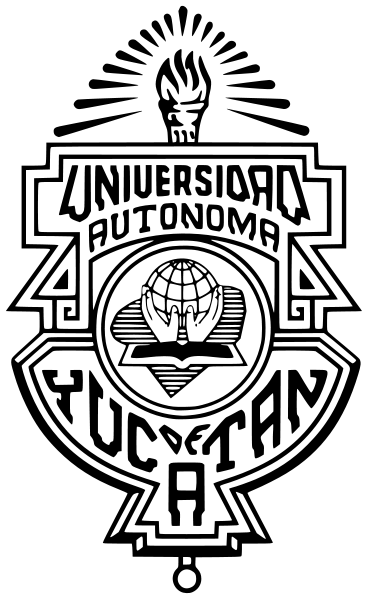
\includegraphics[scale=0.3]{UADY.png}
	\end{figure}}
	\vspace{0.7cm}
	{\Large\itshape Erick Al. Casanova Cortés\par}
	{\Large\itshape Matricula: 15014866\par}
	\vfill
	{\scshape\Large Docente\par
	Dr. O. Carvente\par}
	\vfill
	{\Large{\bfseries Fecha de entrega: 8 Marzo 2021} }

	\vfill
	
\end{titlepage}

%-------------------------------------------------
%Inicio del documento
%-------------------------------------------------


%-------------------------------------------------
%Instrucciones
\section*{Instrucciones}
Redactar un ensayo de las secciones:\\
12-1 Corrientes y densidades de corriente\\
12-2 La ecuación de continuidad\\
12-3 Corrientes de conducción

%-------------------------------------------------
%Corrientes y densidades de corriente
\section*{Corrientes y densidades de corriente}

Como una primera aproximación se puede definir como corriente como la carga que pasa a través de un punto, el cual puede verse interpretado como la corriente promedio $\bar{I}$, por la cual pasa un $\Delta q$ a través de un $\Delta t$, o 

\begin{equation}
	\bar{I} = \frac{\Delta q}{\Delta t}
	\label{eq:corriente_promedio}
\end{equation}

En cambio, si el flujo de cargas no es uniforme en el tiempo habrá que hacer una modificación en la definición de (\ref{eq:corriente_promedio}) a modo que se plantea una corriente instantánea $I$, la cual se define como:

\begin{equation}
	I = \frac{\dd{q}}{\dd{t}}
	\label{eq:corriente_instantanea}
\end{equation}

\begin{figure}[!h]
	\centering
	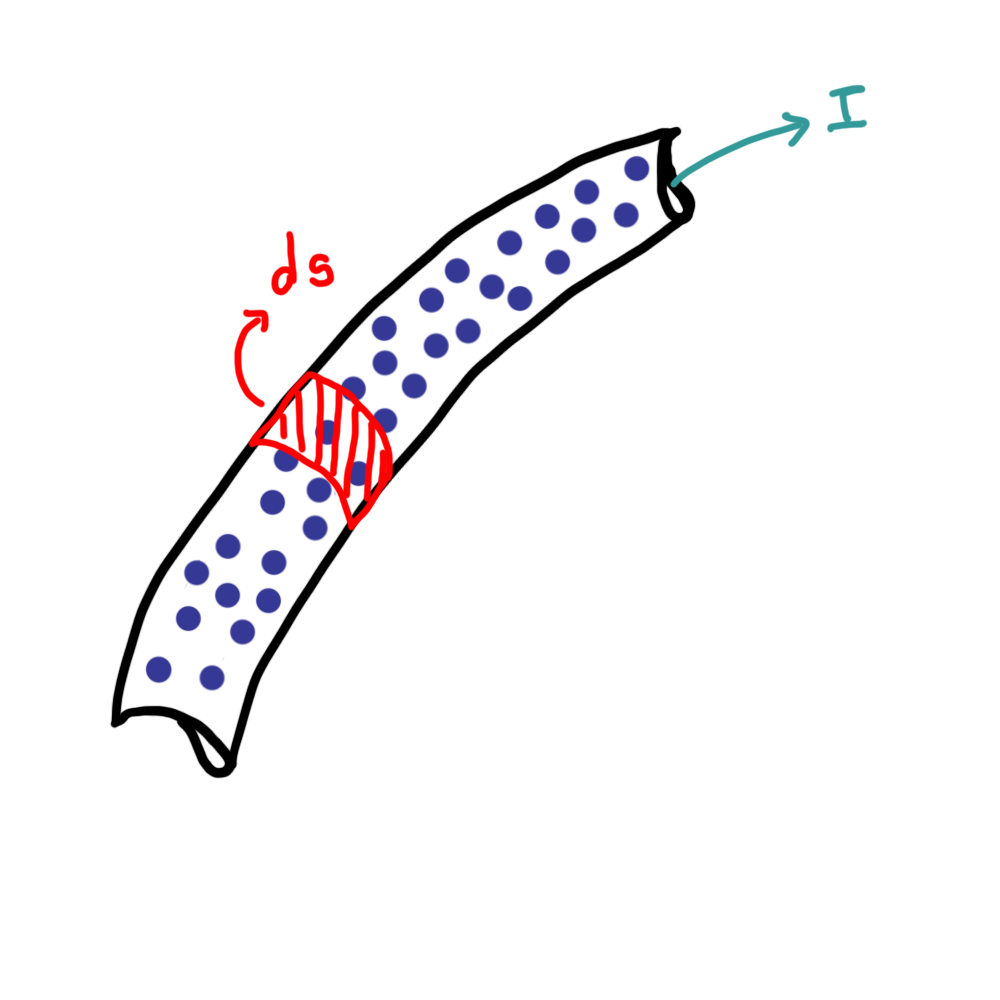
\includegraphics[scale=0.15]{corriente_instantanea}
	\caption{Paso de cargas sobre un cuerpo}
	\label{fig:corriente_instantanea}
\end{figure}


Si analizamos el fénomeno se puede ver a cierta forma como se muestra en la figura \ref{fig:corriente_instantanea}, como se puede ver, las partículas pasan a través del cuerpo, y se toma un diferencial para seguir su trayectoria. Esto es con fines explicativos, ya que podría generar ruido el usar un $\dd{s}$ en un volumen, por lo que a menudo es conveniente pensar que la corriente viaja a lo largo de alguna curva, entonces el $\dd{s}$ es el desplazamiento a lo largo de dicha línea en el sentido de $I$, dicha definición toma el nombre de corriente filamental, aunque como es de esperarse el flujo de las cargas pueden estar distribuidas en un volumen o en una superficie.\\

Entonces es necesario hablar sobre las distintas distribuciones de carga, estas pueden ser volumétricas, superficial o filamental. La densidad volumétrica se define como $J$ y tiene la misma dirección del flujo

\begin{equation}
	\dv{q}{t} = J \cdot \dd{a}
	\label{eq:corriente_vol}
\end{equation}


\begin{equation}
	\dv{q}{t} = |K \cdot \hat{t}| \dd{s}
	\label{eq:corriente_sup}
\end{equation}	
	
	
\begin{equation}
	\dv{q}{t} = \lambda|v|
	\label{eq:corriente_fil}
\end{equation}


La ecuación \ref{eq:corriente_sup} habla del flujo de carga que pasa sobre una superficie, donde $K$ se define como la densidad superficial de corriente, la ecuación \ref{eq:corriente_vol} es sobre el flujo de carga que pasa sobre un volumen, y como se vio previamente $J$ s la densidad volumétrica de flujo, por último está \ref{eq:corriente_fil}, la cual es sobre la corriente filamental, donde $\lambda$ es la densidad lineal de carga de flujo
%-------------------------------------------------
%La ecuación de continuidad
\section*{La ecuación de continuidad}

Si se tiene un volumen limitado por una superficie cerrada, podemos ver que tanto como la superficie y el volumen son constantes, así como la carga del mismo. Por lo mismo es factible decir que la cantidad de carga que entra o sale del volumen es la misma. Por lo que si $Q$ es la carga total del volumen $V$ se tiene que:

\begin{equation}
	-\dv{Q}{t} = \oint_A J \cdot \dd{A}
\end{equation}


\begin{figure}[!h]
	\centering
	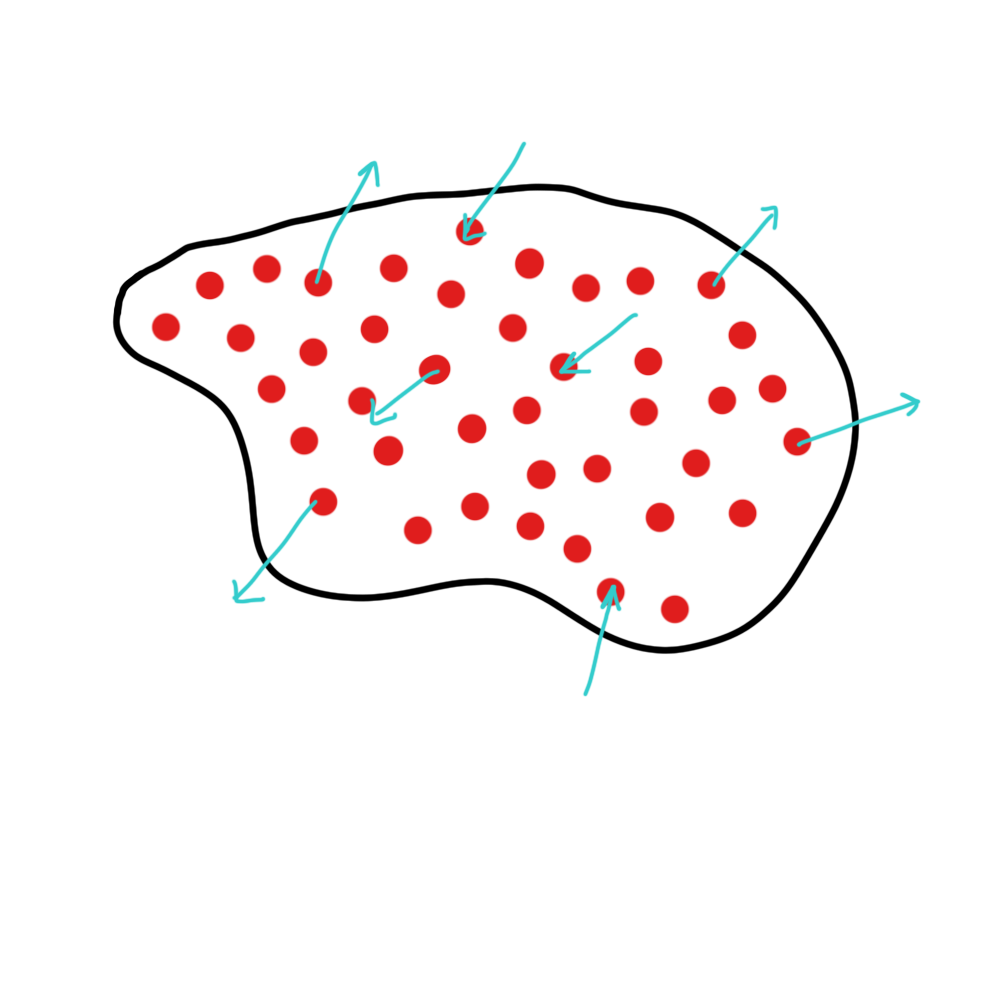
\includegraphics[scale=0.15]{ecuacion_continuidad.png}
	\caption{Volumen limitado con cargas}
	\label{fig:ecuacion_continuidad}
\end{figure}


y como sabemos que $Q = \int \rho \dd{\tau}$, donde $\dd{\tau}$ es la diferencial de volumen; por el teorema de Gauss podemos ver entonces que:

\begin{align*}
	\oint_A J \cdot \dd{A} &= \int \nabla \cdot J \dd{\tau}\\
	-\pdv{t}\int \rho \dd{\tau} &= \int \nabla \cdot J \dd{\tau}
\end{align*}

\begin{align*}
	\int \left( \pdv{\rho}{t} + \nabla \cdot J \right) \dd{\tau} &= 0\\
	\pdv{\rho}{t} + \nabla \cdot J &= 0
\end{align*}

La cual es la ecuación de continuidad.
%-------------------------------------------------
%Corrientes de conducción
\section*{Corrientes de conducción}

Se ha visto que si se aplica una diferencia de potencial a un conductor se generan corrientes en él y estas se mantienen hasta se que retire dicho potencial, haciendo que el conductor llegue a su equilibro electrostático.\\
También se encuentra que es posible mantener una corriente constante en un conductor por medio de una diferencia de potencial constante (suministrando la energía continuamente desde una fuente eterna). Esto es un trabajo realizado sobre estas cargas, entonces si definimos a dicho trabajo como $W_q$ sobre la carga $q$, esta relación recibe el nombre de fuerza electromotriz (fem) $\xi$, la cual se obtiene de la manera

\begin{align*}
	\text{fem} &= \xi\\
	\xi &= \frac{W_q}{q}\\
	&= \oint_c \frac{F_q \cdot \dd{s}}{q}\\
	&= \oint_c E\cdot\dd{s}
\end{align*}

Dado que se ejercerán fuerzas sobre las cargas en movimiento, deberá existir cierta relación
funcional $J$ y $E$ debe tener una relación cual que:

\begin{equation}
	J = J(E)
\end{equation}

%-------------------------------------------------
%Final del documento
%-------------------------------------------------

\end{document}
